\newpage
\chapter{Introduction}
\label{sec:introduction}
\section{Action Recognition on First-Person Video}
\label{sec:action-recognitions}
\blue{First person point of view video is a video produced by egocentic camera that capture the scene with a first person perspective. By installing an egocentric camera like GoPro  or Google Glass,  people can easily record egocentric video. For example, as shown in Figure \ref{fig:dogcentric}, egocentric videos captured by mounting the camera on the head of the animal such as a dog.}

\blue{Increasing the number of egocentric cameras is directly proportional to the availability number of first-person video. This causes a phenomenon in the field of computer vision, in which the researcher is interested in studying and analyzing more deeply to provide more usefulness in daily life. For example, the use of first-person camera in the military, where soldiers dressed in smart helmet with egocentric vision to assist them in analyzing the movements of the enemy in battle. It can also be applied to the world of robots, where robots can identify movement or action of his opponent so they can have a better communication. Furthermore, it can be applied to the self-driving car to recognize movement patterns recorded in front of the car. For example, if there is an accident or a sudden movement from unknown subject passed right in front of him. It is evident many such applications that require recognizing the activity of camera wearer as an essential first step.}

\blue{For first-person (egocentric) videos, the which are recorded by the model's view point,} in general features are rich in noise and contain plenty of uncontrolled variations scene. Moreover, these videos need to deal with some adverse effects such as shaky frame, background clutter, occlusion and inter-class variation.
\blue{Coupled with the absence of the actor's pose, it makes the first-person video is more challenging than the third person video. In contrast to the third person that video recorded with less motion, on a first-person video, the camera also moves to follow the movement of the actor's head. So the extreme change of viewpoint making the system difficult to track the movement with tracking algorithm that currently exists for a third-person video.}
Consequently, it is a challenging task to find an effective and
robust feature representation for first-person videos.
Fig. \ref{fig:different} shows the difference between first-person and third-person video. 

\begin{figure}[!t]
	\centering
	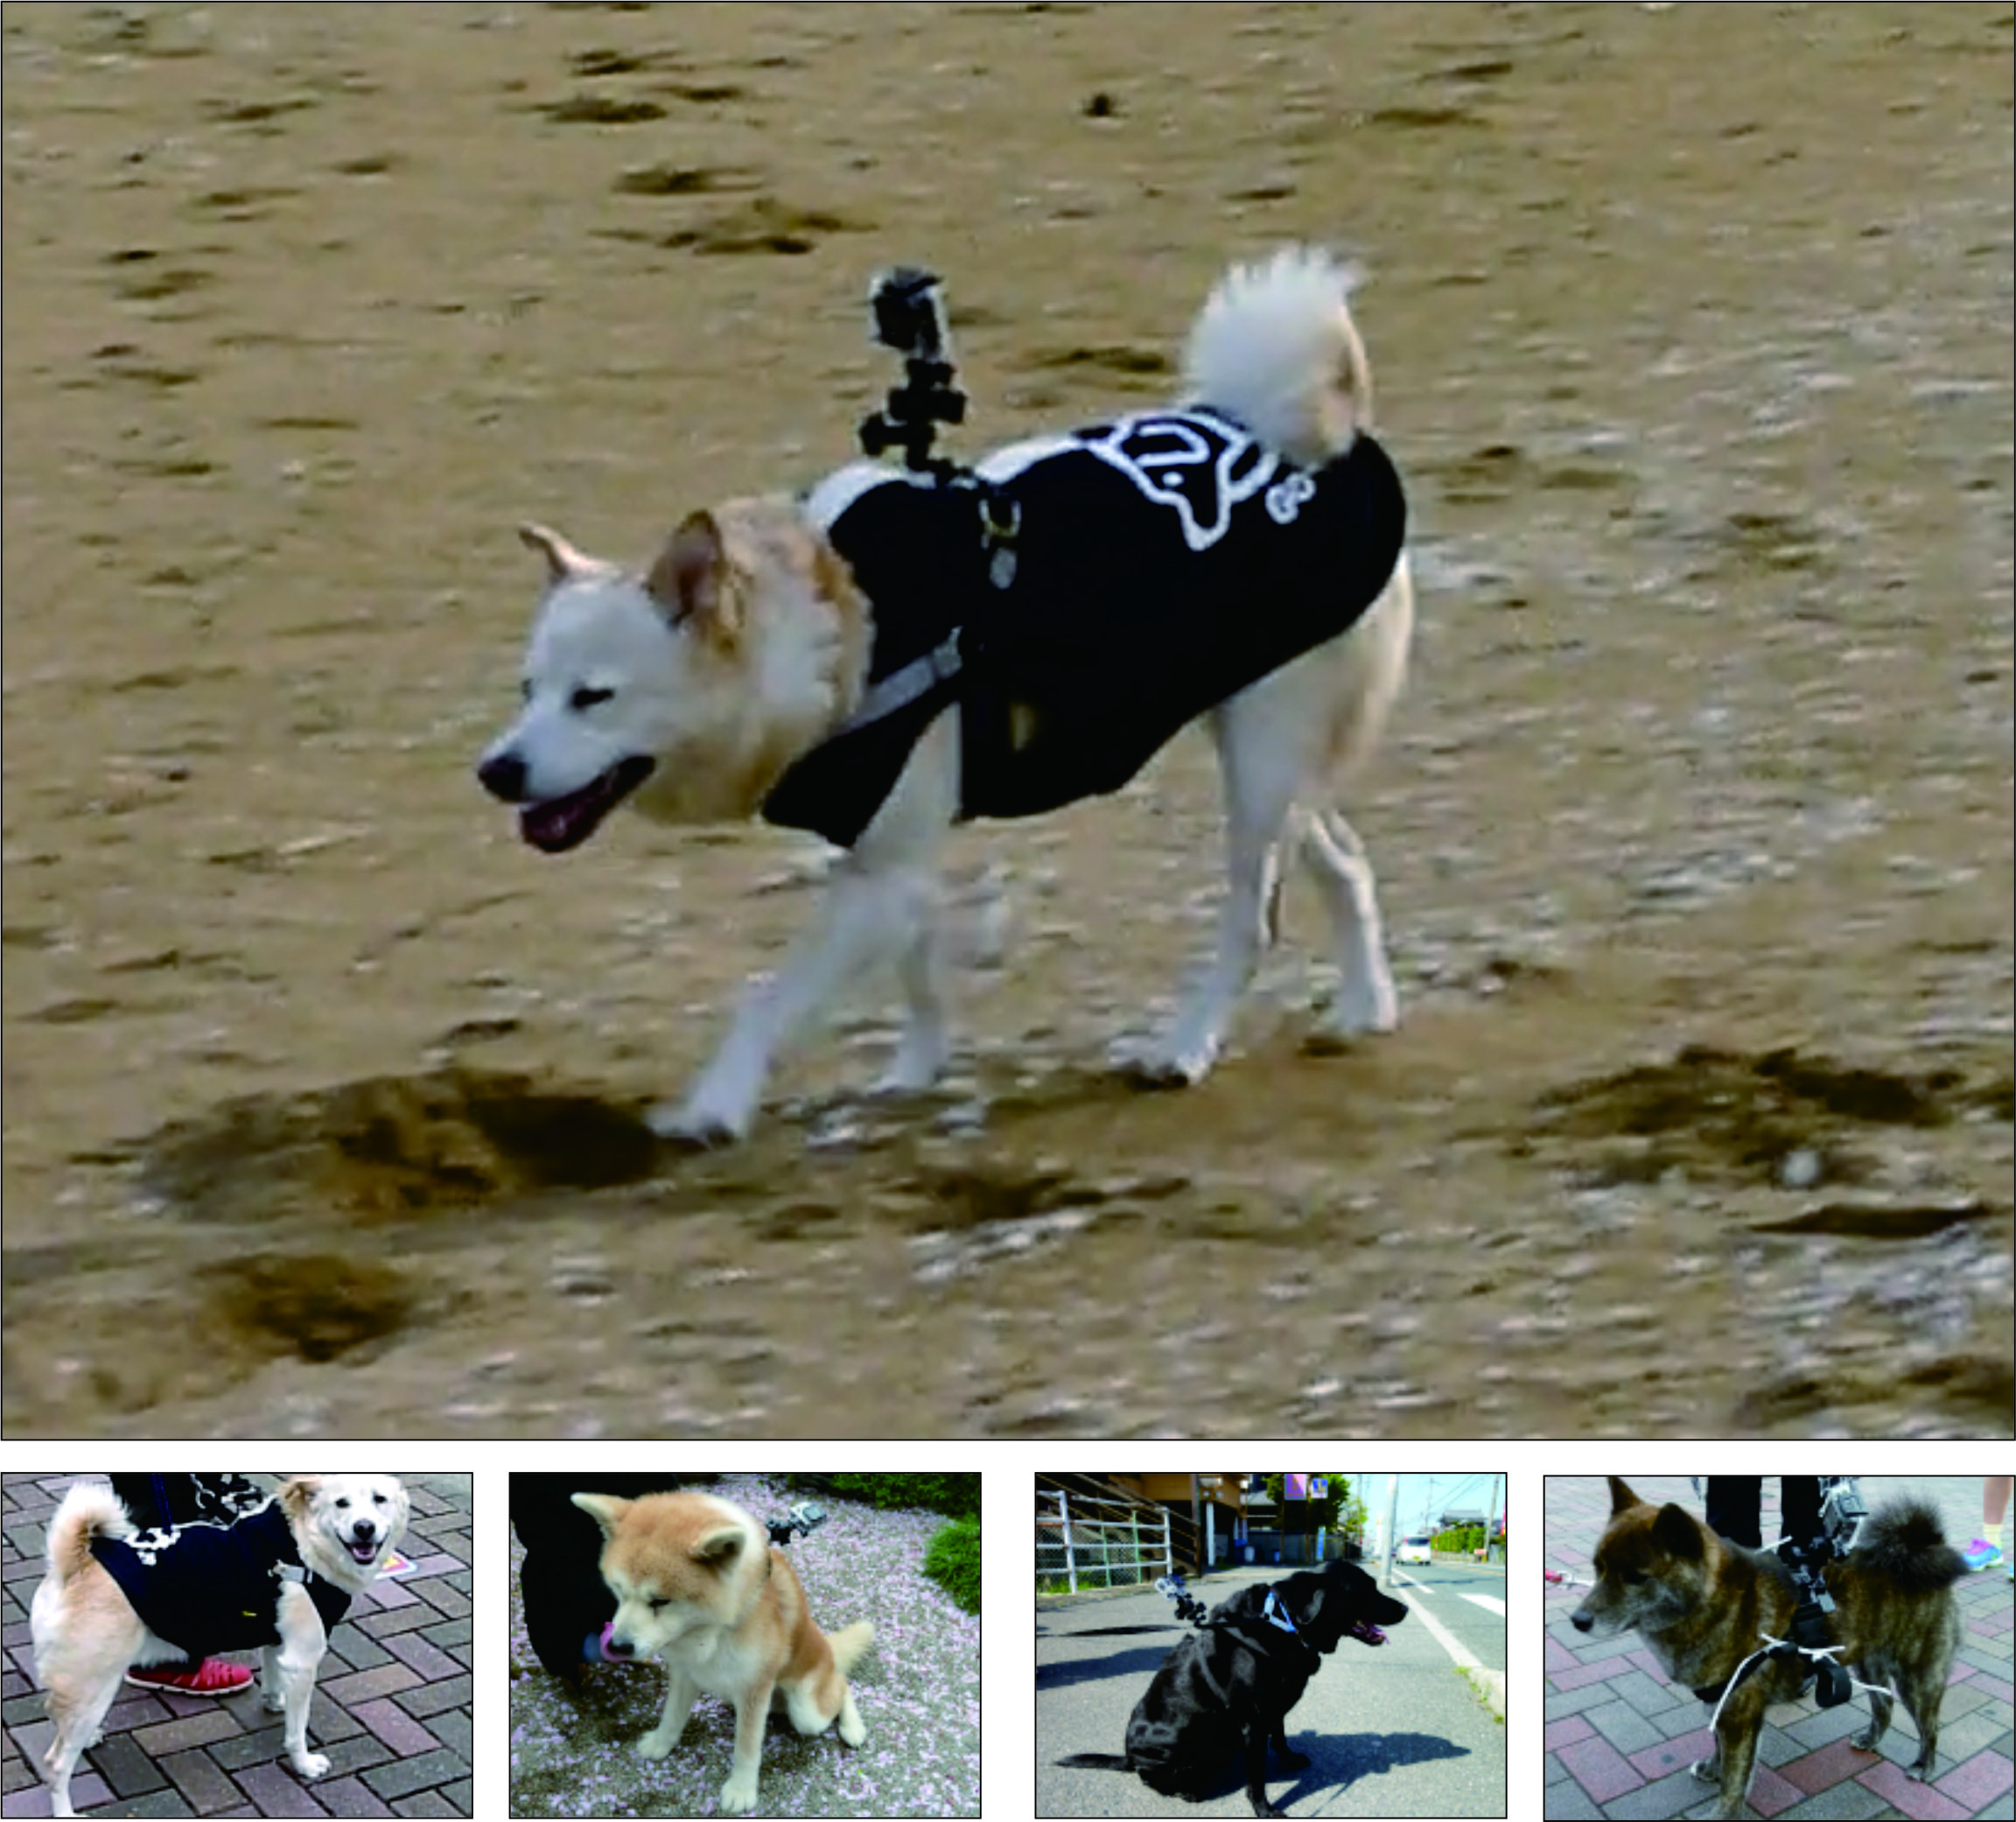
\includegraphics[width=0.8\textwidth]{figures/dogcentric}
	\caption{Egocentric cameras such as GoPro is typically mounted on the head of the dog in DogCentric dataset. This camera capture the action from first-person point of view. 
	} 
	\label{fig:dogcentric}
% 	\vspace{-4mm}
\end{figure}

A myriad of algorithms has been proposed  for action recognition in
videos, including local spatio-temporal  descriptors such as dense
trajectories \cite{wang2013dense}, \cite{wang2011action} and improved dense trajectories \cite{wang2013action}, and convolutional neural network
(CNN) based approach \cite{wang2015action}, \cite{simonyan2014two}, \cite{wang2015temporal}. However, those methods are not specifically
devised for  the first-person videos and thus in general can not provide
satisfactory detection performance in this scenario. Recently, some
approaches were suggested for the first-person action recognition. For
instance, Iwashita \textit{et al.} \cite{iwashita2014first} used the
conventional local and global motion descriptors and clustered them
into visual words. Ma \textit{et al.} \cite{ma2016going} addressed a
two-steam ConvNet architecture which incorporated both spatial and
temporal networks. However, it only considered the temporal
characteristics of videos and demanded a large number of training
samples. Ryoo \textit{et al.} \cite{ryoo2015pooled} tracked the
changes of the descriptor values by pooled time series. It,
however, only considered simple pooling strategies and some
important temporal information may be lost. Recently
Kahani \textit{et al.} \cite{kahani2016time} grouped the time series
feature and computed the linear correlation among these groups.
However, it requires a judicious  selection of the local time
windows.

In light of the non-stationary nature of the feature vectors, in
this \blue{thesis}, we, inspired by the success of Hilbert-Huang transform
(HHT) \cite{huang1998empirical} in EEG, ECG, %MEG
and other non-stationary signal analyses \cite{xie2006mean},
\cite{echeverria2001application}, consider a new method which aggregates
both of the short- and long-term trends based on the coefficients of
HHT. To achieve this, we apply HHT to the trajectory-pooled
deep-convolutional descriptors (TDD) \cite{wang2015action},
which includes both of the trajectory information
\cite{wang2013action}
and the deep-learned features \cite{simonyan2014two}, and treats the temporal dimension as feature channel.
HHT decomposes the TDD feature vector in each channel via a set of intrinsic mode
functions (IMFs) based on the empirical mode decomposition (EMD) and
then analyze the coefficients using Hilbert transform. Thereafter,
some  characteristics of the coefficients \cite{riaz2016emd} are
determined to render more precise feature representation.


To the authors' best knowledge, it is the first time HHT is employed
for action recognition in videos. This new approach possesses
several salient features. First, it can prune out noisy feature
channel by selecting an appropriate IMF combination through EMD.
Second, it can take both of the short- and long-term trends of the
video into consideration to render better understandings of
the trends or patterns of the features in the first-person videos.
The proposed approach can also be successfully incorporated with the
CNN features such as trajectory pooled CNN features to
achieve superior detection accuracy. Simulations show that
the proposed method outperforms the main state-of-the-art works on
two widespread public first-person datasets.



\begin{figure}[!t]
\centering
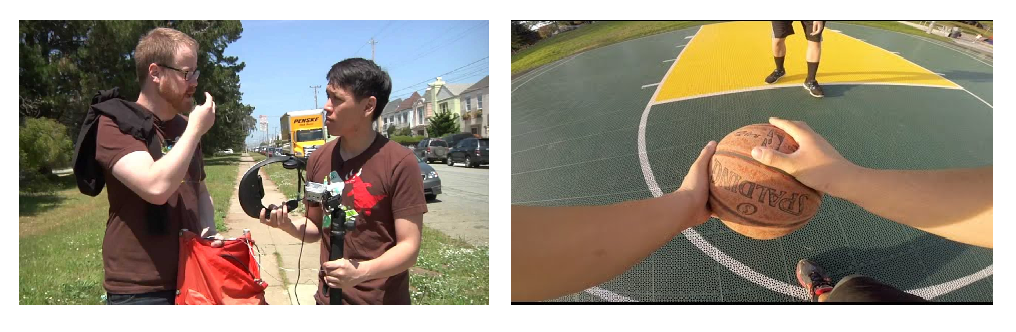
\includegraphics[width=0.85\textwidth]{figures/1s}
\caption{Differences in viewpoint in the first person to third person video videos. The left figure is the characteristic of the third person video, while the right figure is the characteristic of the first-person video.
} 
\label{fig:different}
%\vspace{-4mm}
\end{figure}


\section{Scope of this thesis}

\subsection{Problem Statements and Challenge}
\label{sec:problem-statements}
\blue{We focus on action recognition in the first-person/egocentric videos. The main challenge in this work are camera motion and wild motion caused by wearer's natural head motion which make video so shaky that hard to be analyzed. Also, the background also moving in the first-person video make the system hard to separating between foreground and background.}

\blue{Usually by determining the foreground object first, we can make our best representation descriptor. But, since the characteristic of the first-person video that background also moving, sometimes make the background be  important component to be extracted as foreground. }
	
\blue{We observe that in any egocentric video involving sub-action that move in the same time. We found that saliency image can benefit the system to make best feature descriptor. By extracting optical flow from two consecutive images, then applying some thresholds to obtain new saliency motion map representation, we can detect the fine-grained object and select the feature around it. We assume that the features extracted from fine-grained object is more important than the feature extracted from sub-objects.
We also focus on short-time term actions that typically last few seconds, e.g., pour, take, open etc. 
Fig. \ref{fig:kitchen} gives some examples of the actions we are interested in recognizing.}

\begin{figure}[!t]
	\centering
	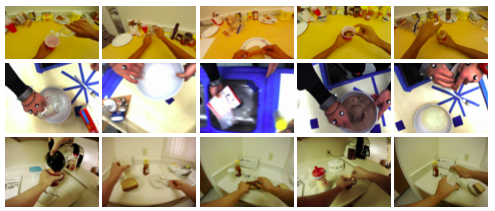
\includegraphics[width=0.95\textwidth]{figures/kitchen}
	\label{fig:kitchen}
	\caption{The action which we aim to recognize.
	} 
	%\vspace{-4mm}
\end{figure}

\blue{We also observe that frame selection is important task to increase the detection performance. Given a video, which consist of a lot of similar consecutive frames. Those similar consecutive images will produce the duplication of the descriptor, which influence the quality of the feature representation. Hence, the scheme need to be developed to circumvent this situations. 
We observe to do frame selection as preprocessing step. Given a video consists bunch of images, we pool them into sequel of time window. Then, we identify the most essential frame by performing pooling on the SVM.}

\blue{Convolutional neural network ($CNN$) which popular nowadays in many area can be useful tool for computer vision task. However, it produce a huge number of descriptor. We show that simple pooling strategy is not enough to deal with this, hence we employed non-stationary tool analysis, Hilbert-Huang Transform to aggregates the descriptor into one representative feature video.}

\blue{Furthermore, the datasets that we use in this work are very challenging. The characteristic of these three datasets are different each other. The first dataset, DogCentric dataset \cite{yumi2014first} is the most difficult one since the video recorded in dog head. This dataset is the shakiest dataset that we used in this thesis. The second dataset is JPL dataset \cite{ryoo2013first}, which use a doll as a model. The typical of this dataset is the interaction dataset. People will interact with the model in some action like hug, wave, punch, etc. While the last dataset \cite{spriggs2009temporal} is continues dataset which recorded in long period of time. Unbalanced number of video and the rough label annotation make the action classification even more harder.}


\subsection{Contributions}
\label{sec:contributions}
\blue{We propose a temporal aggregation for first-person video using non-stationary tools, Hilbert-Huang Transform. To the best author's knowledge, it the first time non-stationary tools used for temporal aggregation in computer vision area. We also perform background-foreground separation by selecting only the inlier trajectory. Also, the frame selection in the first part has increased the performance of detection. We have explored the generalization of our proposed method by performing in three different characteristics first-person point of view video. We show later that our technique can corporate with $CNN$ features and improve it performance. 
This work proposes a general temporal aggregation for first-person action recognition with following specific contributions:
}
\blue{
\begin{enumerate}
	\item We propose new temporal aggregation technique for first-person video by using Hilbert-Huang transform (HHT). To the best of author's knowledges, this is the first-time that HHT employed for action recognition in video.
	\item We propose dominant motion saliency object and its trajectory to select inlier trajectories to prune the noisy features caused by camera moving in first-person video.
	\item Our feature representation can prune out noisy feature
	channel by selecting an appropriate IMF combination through EMD. Also, Our feature can take both of the short- and long-term trends of the
	video into consideration to render better understandings of
	the trends or patterns of the features in the first-person videos.
	\item We propose frame selection in the preprocessing part to improve the detection performance.
    
\end{enumerate}
}
\section{Thesis Outline}
\blue{Brief outline of text in this thesis is as follows. In chapter 2, we review of the related work. In chapter 3, we explain our contributions on the proposed approaches for first-person action recognition which is temporal aggregation using Hilbert-Huang transform. In chapter 4, we explain our experimental and result. 
Finally, we end the thesis with concluding remarks and future work.} 


